\chapter{Instructions for Installation}

\section{Checking out the files}
After you have started Eclipse 3.0, change to CVS Repositories perspective and add a CVS repository. \par
Enter the following data (see \ref{neuesrep}):
\begin{itemize}
\item host: cvs.berlios.de
\item repository path: /cvsroot/kobold
\item user: anonymous
\end{itemize}
Leave the remaining data untouched and confirm the dialog. \par

\begin{figure}[h!]
\begin{center}
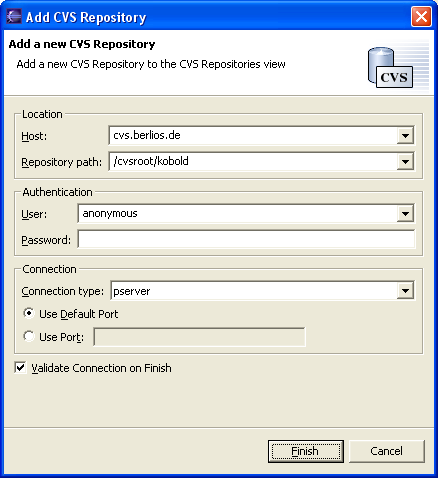
\includegraphics[width=12cm]{neuesrep.png}
   \caption{Adding a new repository}�
\label{neuesrep}
\end{center}
\end{figure}

Open the tree along HEAD, kobold and src (see \ref{auschecken}). Check out the five folders kobold.client.plam,
kobold.client.vcm, kobold.client.serveradmin, kobold.common and kobold.server through 'check out as..' (context menue)
and confirm with 'Finish'.

\begin{figure}[h!]
\begin{center}

\includegraphics[width=10cm]{auschecken.png}
   \caption{This is how your tree should look like}
\label{auschecken}
\end{center}
\end{figure}\par

Open the 'Window' menu and select 'preferences'. Select 'plug-in development' and 'Target 
Platform' and press the button 'Not in Workspace'. Confirm with OK. \par

Projects kobold.client.plam, kobold.client.vcm and kobold.common: \par
Right-click on the project and select 'properties'. Select 'Java build path' and the 'source'
tab. Remove the existing entry and add a new one by pressing 'Add Folder'. Choose the 
src-folder and confirm. Append '/bin' to the default output folder (see \ref{buildpath}).
 Close the preferences dialog. \par

\begin{figure}[h!]
\begin{center}
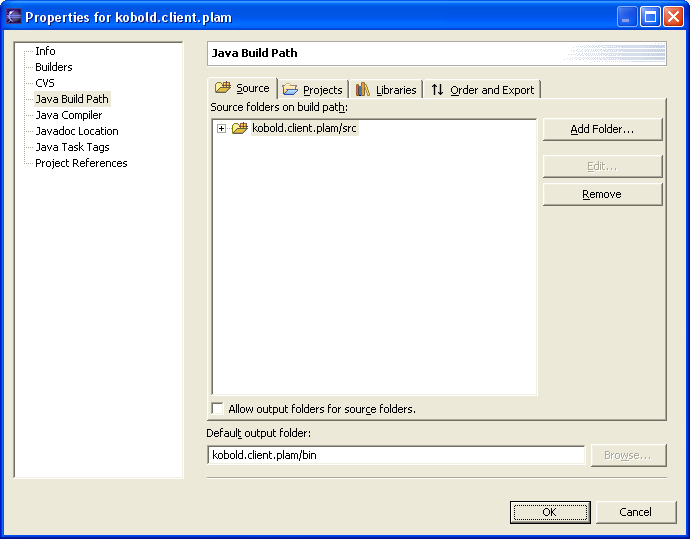
\includegraphics[width=15cm]{buildpath.png}
   \caption{This is how your buildpath should look like}
\label{buildpath}
\end{center}
\end{figure}\par

Projects kobold.server: \par
Right-click on the project and select 'properties'. Select 'Java build path' and the 'source'
tab. Remove the existing entry and add a new one by pressing 'Add Folder'. Choose the 
src-folder and confirm. Append '/bin' to the default output folder. 
Switch to the 'projects' tab and select 'kobold.common'. Close the preferences 
dialog. \par

Again, right-click on the project kobold.client.plam and select 'PDE Tools' 
and then 'update classpath'. Select 
kobold.client.plam, kobold.client.vcm and kobold.common and confirm.

\section{Setting the correct properties}


First of all edit the server.properties
file from {\it kobold.server/server.properties} to suite your local
requirements. Under UNIX this file might look similiar to the following
bits:

\begin{verbatim}
# Note storePath is the prefix path for all kobold stores!
kobold.server.storePath=/tmp/
kobold.server.globalMessageStore=global.xml
kobold.server.messageStore=messages.xml
kobold.server.productStore=product.xml
kobold.server.userStore=user.xml
#
java.protocol.handler.pkgs=com.sun.net.ssl.internal.www.protocol
javax.net.debug=all
javax.net.ssl.keyStore=../kobold.common/scripts/keystore
javax.net.ssl.keyStorePassword=kobold1
javax.net.ssl.trustStore=../kobold.common/scripts/truststore
javax.net.ssl.trustStorePassword=kobold1
\end{verbatim}

Under Windows-based systems you've to change the paths into a
DOS-alike format.

In the following table all properties are described in detail:

\begin{tabular}{|l|l|l|}\hline
\textbf{Property} &  \textbf{Description}\\ \hline
kobold.server.storePath  & destination path for files stored by the server \\ \hline
kobold.server.globalMessageStore & file name to store global messages \\
    \hline
kobold.server.messageStore & file name to store pending messages \\
    \hline
kobold.server.productStore & file name to store products and
productlines \\ \hline
kobold.server.userStore & file name to store user data \\ \hline
java.protocol.handler.pkgs & default protocol to commincate \\ \hline
javax.net.debug & debug level of net communication \\ \hline
javax.net.ssl.keyStore & path to your SSL keystore \\ \hline
javax.net.ssl.keyStorePassword & password to access your SSL keystore \\
    \hline
javax.net.ssl.trustStore & path to your SSL truststore \\ \hline
javax.net.ssl.trustStorePassword & password to access your SSL
truststore \\ \hline
\end{tabular}

You also have to edit the sat.properties file from {\it kobold.client.serveradmin/sat.properties} 
to suite your local
requirements. Under UNIX this file might look similiar to the following
bits:

\begin{verbatim}
#used to communicate with Kobold servers via ssl
java.protocol.handler.pkgs=com.sun.net.ssl.internal.www.protocol
javax.net.debug=all
javax.net.ssl.keyStore=/home/garbeam/eclipse/kobold.common/scripts/keystore
javax.net.ssl.keyStorePassword=kobold1
javax.net.ssl.trustStore=/home/garbeam/eclipse/kobold.common/scripts/truststore
javax.net.ssl.trustStorePassword=kobold1
\end{verbatim}

As you can see, it contains the same properties as the {\it
server.properties} file for SSL communication, but since the Kobold
client is independent from the server it has its own properties.\par

Right after your first start of the Kobold Client Feater Set, change the Kobold
preferences so that the client-server communication works properly. For more
information go to the tutorial section.